\documentclass[aps,pra,10pt,twocolumn]{revtex4-2}
% revtex4-2 = version 2 of the review text class
% aps       = American Physical Society (society type)
% pra       = Physical Review A (journal type)
% 10pt      = font size
% twocolumn = true

\usepackage{silence} % NB: put *before* package you want to silence
\WarningFilter{caption}{Unknown document class} % Caption package does not support revtex4

\usepackage{times} % Times New Roman

\usepackage[a4paper, left=1.85cm, right=1.85cm,top=1.85cm, bottom=1.85cm]{geometry}

% Defines caption font size as 9pt and caption title bolded
\usepackage[style=base, font=small, labelfont=bf]{caption}
\usepackage{subcaption}

\usepackage{graphics,graphicx,epsfig,ulem}  % Graphics package
\usepackage{amsmath} 						% Maths package

\usepackage{siunitx} % SI units, alignment in tables

\usepackage{lipsum}
\usepackage[british]{babel} % British date system

\usepackage{multirow} % Multirow cells in tables
\usepackage{booktabs} % Nice table separators

\usepackage{hyperref} % For hyperreferences


% Customise date to preferred format
\usepackage{etoolbox}
\makeatletter
\patchcmd{\frontmatter@RRAP@format}{(}{}{}{}
\patchcmd{\frontmatter@RRAP@format}{)}{}{}{}
\renewcommand\Dated@name{}
\makeatother

\usepackage{fancyhdr}
\pagestyle{fancy}                           % Insert header
\renewcommand{\headrulewidth}{0pt}
\lhead{L.\ Kirby}                           % Header name
\rhead{Towards the automatic arrangement of music via quantum annealing}            % Header title              

\def\bibsection{\section*{References}}      % Defining bibsection
 
\begin{document}

\title{Towards the automatic arrangement of music via quantum annealing}
\author{L.\ Kirby}                              % Author
\affiliation{\normalfont Durham University}                % Subtitle
\date{Submitted: \today{}}     % Date

\begin{abstract}              

\lipsum[1]

\end{abstract}

\maketitle

\thispagestyle{plain} % Produces front page number

\section{Introduction} 

% Motivation for report, existing literature


\section{Theory} 

% Understanding of physical problem.

\begin{equation}
    f(E)=\begin{cases}
        1\qquad & E\le E_F \\
        0\qquad & E>E_F
    \end{cases}
\end{equation}

\begin{equation}
    E_F=\frac{k_F^2}{2m_e} \,.
\end{equation}


\section{Degenerate case}

%Identify most important results clearly and convincingly
%Shows that computer code works correctly (numerical convergences, systematic errors, random errors, etc.)

\begin{figure}[h]
    \centering
    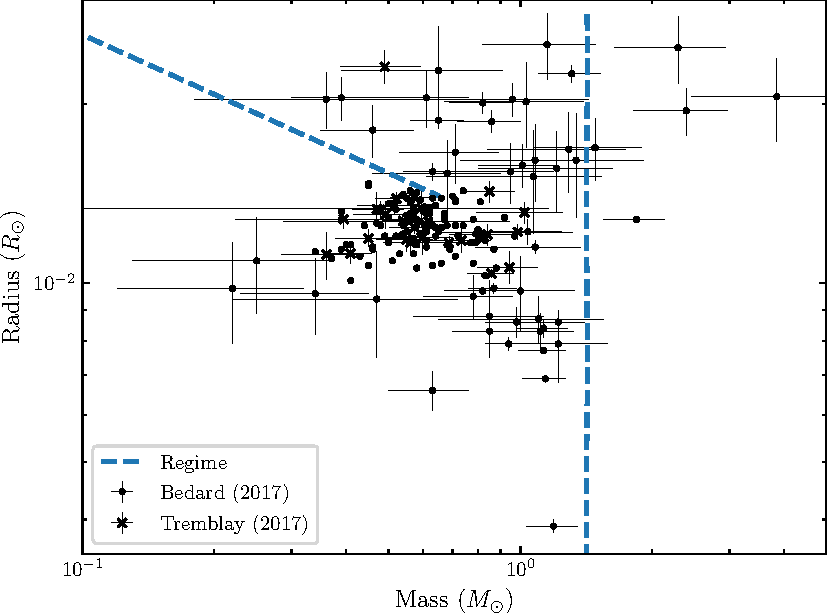
\includegraphics[width=\linewidth]{images/regime-model.pdf}
    \caption{}
    \label{fig:regime}
\end{figure}

% Physical implication of results
% Does code work? Comparison to literature, tests (IMPORTANT)
% Demonstrate student's contribution and motivation

\section{Corrections}

\begin{table}[ht] % Table environment specifies caption, label, location
    \caption{Summary of frational changes to best-fit parameters due to electron energy density and electrostatic corrections.}
    \label{tab:corrections}
    \setlength{\tabcolsep}{12pt} % Column spacing
    \renewcommand{\arraystretch}{1.5}
    \begin{tabular}{c|c|c|c} % S aligns to decimal point
        \toprule
        \textbf{Correction} & $|\Delta A|/A$ & $|\Delta B|/B$ & $|\Delta q|/q$\\
        \midrule
        $\varepsilon_\mathrm{elec}$ & 0.026 & 0.0031 & 0.0442 \\
        $p_c$ & 0.009 & 0.0114 & 0.0005 \\
        \bottomrule
    \end{tabular}
\end{table}

\section{Non-degenerate limit}

\begin{align}
    p&=\frac{\hbar c}{12\pi^2}\left(\frac{3\pi^2}{m_n c^2\eta}\right)^{4/3}\left[\frac{1+2d(S_e)^2+\frac{7}{15}d(S_e)^4}{(1+d(S_e)^2)^{4/3}}\right]\varepsilon^{4/3}\\
    &=\bar{K}(S_e)\varepsilon^{4/3} \,.
    \label{eq:nondegeos}
\end{align}

\section{Conclusions}

%Present ideas for further investigation

The study of white dwarfs is very much ongoing research, with new models arising with the advancement of computational power and new satellite observations that test these models. It is incredible that an investigation such as this, through the application of fundamental statistical physics and computer modelling, can attempt to understand the nature of stellar remnants that seem so unreachable.

\nocite{*}
\bibliographystyle{unsrt}\bibliography{interim}

\clearpage

\onecolumngrid % Puts summary into single column

\section*{Scientific Summary for a General Audience}

\lipsum[1]

\end{document}